\documentclass[conference]{IEEEtran}
\usepackage{amsmath,graphicx,url,array,booktabs}
\usepackage[hidelinks]{hyperref}
\hypersetup{pdftitle={Card Fraud Triage - Phase 2},pdfauthor={Team T011}}
\graphicspath{{../figures/}}
\title{Card Fraud Triage via Gaussian Mixture Density Scoring and Autoencoder Anomaly Detection\\Phase 2: Deep Learning and Score Fusion}
\author{\IEEEauthorblockN{H Maheshwari, Vaibhav, Mayank, Keshav, Mitul Bhatia}
\IEEEauthorblockA{Team T011, Section A, Project 26\\Newton School of Technology, Rishihood University\\
2401010174, 2401010486, 2401010267, 2401010222, 2401010279}}
\begin{document}
\maketitle
\begin{abstract}
We extend our Gaussian Mixture Model (GMM) fraud-triage baseline with a small denoising autoencoder (AE). Both models learn from the same 169,893 earlier legitimate transactions and score the same later mixed test period. We also implement fixed equal-weight fusion of normalized density and reconstruction scores. On 56,746 test transactions containing 74 frauds, trapezoidal precision-recall area is 0.1496 for GMM, 0.1308 for AE and 0.1412 for the hybrid. The top 100 reviews find 29, 24 and 25 frauds respectively. At the default 0.5\% validation false-positive policy, the hybrid finds 35 frauds with 132 false alerts, compared with the GMM's 37 with 172. Thus fusion improves the AE and changes the false-alert trade-off, but does not beat the GMM's overall ranking. Noise, bottleneck size, a second random seed and linear reconstruction ablations expose important limitations. Phase 1 already exposed the test benchmark; this is a consistent reused-benchmark comparison, not a new blind test.
\end{abstract}
\begin{IEEEkeywords}fraud triage, anomaly detection, autoencoder, Gaussian mixture, score fusion\end{IEEEkeywords}

\section{Problem and Phase 2 Objective}
Fraud triage orders transactions for human review. An anomaly is a reason to investigate rather than proof of fraud. Rare positives make accuracy an inadequate headline: always predicting legitimate would achieve about 99.87\% test accuracy while finding no fraud. We instead measure precision-recall (PR) ranking, recall at validation false-positive rate (FPR) budgets, and precision at a fixed review capacity.

Phase 1 modeled normal transaction density with a GMM. Phase 2 asks whether nonlinear reconstruction captures useful information missed by that density model. Our hybrid is an implemented score-fusion rule, not merely a side-by-side comparison. Its value must be demonstrated by ablation and measured trade-offs, as required by the supplied course instructions. We do not claim a new algorithm or guaranteed additional marks.

\section{Related Work and Motivation}
Dempster, Laird and Rubin~\cite{em} provide the EM framework underlying mixture estimation. Our frozen baseline retains Phase 1's diagonal-covariance GMM and AIC/BIC component study. Better legitimate density fit does not itself establish better fraud ranking.

The assignment recommends Sakurada and Yairi~\cite{sakurada} for AE anomaly detection using nonlinear dimensionality reduction. We use this as motivation for the reconstruction comparison; we do not reproduce its experiments or import its performance claims. Publisher full text was unavailable during preparation, so no detailed experimental assertion is based on that paper.

Vincent et al.~\cite{vincent} study learning representations by recovering clean inputs from corrupted versions. We adapt this clean-target denoising idea to a small jointly trained tabular AE. We do not reproduce the full stacked pretraining procedure or assume its classification findings transfer to fraud anomaly ranking. Our plain-versus-denoising experiment checks the local intervention.

Saito and Rehmsmeier~\cite{pr} motivate examining precision and recall when positives are rare. We also retain operational counts and FPR budgets, since a small FPR can still create many legitimate alerts. Software documentation~\cite{sk,torch} supports the metric and loss implementation. In particular, average precision (AP) and trapezoidal PR area use different integration conventions.

\section{Data and Fair Comparison}
\subsection{Quality, Splits and Base Rates}
The ULB/Worldline dataset~\cite{data} contains 284,807 transactions and 492 frauds, spanning two historical days. We verify the exact CSV SHA-256 against Phase 1 and find no missing or nonfinite values. Following Phase 1, stable time sorting and removal of 1,081 exact repeated rows leave 283,726 rows and 473 frauds. Without transaction IDs we cannot prove every repeated row is an accidental duplicate; removal is a declared preprocessing assumption.

The chronological 60/20/20 split contains 170,235 training rows (342 frauds), 56,745 validation rows (57 frauds), and 56,746 test rows (74 frauds). Corresponding fraud rates are 0.2009\%, 0.1004\%, and 0.1304\%. Only the 169,893 legitimate training rows fit the GMM, AE and linear reference. The label is used to identify known legitimate rows, so this is commonly termed one-class or semi-supervised anomaly detection; the reconstruction objective itself uses no fraud targets.

\subsection{Shared Inputs and Leakage Controls}
Both main models receive V1--V28 and $\log(1+\mathrm{Amount})$, totaling 29 features. Time orders the split but is excluded from the inputs. Class is never an input. StandardScaler fits means and standard deviations on legitimate training rows only; validation and test reuse them unchanged. We check the scaled arrays and row order against the existing Phase 1 arrays. We apply no clipping. Provider anonymization and PCA preparation cannot be independently audited from this CSV.

Legitimate validation rows choose AE checkpoints, score normalization and FPR cutoffs. They never update model weights. No Phase 2 model or hybrid-weight choice uses test labels. Nevertheless, Phase 1 results on this exact test period were already visible, so it cannot serve as a newly blind holdout. All test conclusions are descriptive results on that reused chronological benchmark.

\section{Methods}
\subsection{Frozen GMM Baseline}
For $K$ components, the normal density is
\begin{equation}
p(x)=\sum_{k=1}^{K}\pi_k\mathcal{N}(x\mid\mu_k,\Sigma_k),\qquad s_G(x)=-\log p(x).
\end{equation}
EM alternates membership estimates and parameter updates. Phase 1 fits $K\in\{1,2,4,8\}$ using three starts, seed 42, at most 200 iterations, and covariance regularization $10^{-6}$. All candidates converge. K=8 minimizes training BIC (10,144,915) in this grid. Both AIC and BIC continue falling at its edge; eight is not established as globally optimal. Diagonal covariance reduces parameters but ignores within-component cross-feature covariance. This frozen baseline reproduces Phase 1 PR area to numerical tolerance.

\subsection{Undercomplete Denoising Autoencoder}
Our fully connected network has widths $29,16,8,16,29$ and 1,253 trainable parameters. The encoder compresses to eight units and the decoder reconstructs 29 features. ReLU follows each hidden Linear layer, including the bottleneck. A linear output permits negative standardized targets. The narrow bottleneck discourages direct copying while hidden nonlinearities allow relationships beyond linear reconstruction.

For a clean legitimate input $x$ and corrupted input $\widetilde{x}=x+\epsilon$, with independent $\epsilon_j\sim\mathcal{N}(0,0.1^2)$, the reconstruction objective is
\begin{equation}
\mathcal{L}(\theta)=\frac{1}{29N}\sum_{i=1}^{N}\sum_{j=1}^{29}\left[f_\theta(\widetilde{x}_i)_j-x_{ij}\right]^2.
\end{equation}
At evaluation, inputs are clean and the anomaly score is
\begin{equation}
s_A(x)=\frac{1}{29}\sum_{j=1}^{29}(f_\theta(x)_j-x_j)^2.
\end{equation}
For example, reconstructing $[1,2]$ as $[1.1,1.8]$ yields MSE 0.025. High error suggests reconstruction difficulty, not a fraud probability. Fraud can reconstruct well and rare legitimate activity can reconstruct poorly.

\subsection{Training and Regularization}
Adam uses learning rate 0.001, weight decay $10^{-5}$ and batches of 1,024. Each update corrupts the input, performs a forward pass, computes clean-target MSE, backpropagates gradients and updates weights after clearing old gradients. An epoch is one pass over training rows. Training uses CPU with two threads, deterministic operations and seed 42.

We evaluate clean training and legitimate-validation MSE after each epoch. The best accepted improvement exceeds $10^{-4}$. We restore that checkpoint and stop after five epochs without improvement or at 30 epochs. Compression, noise, weight decay and stopping constrain training. The main architecture and settings are fixed in advance rather than selected for test fraud ranking. Both plain and main denoising AE reach epoch 30 and restore epoch 30. The wider model stops after 15 epochs and restores epoch 10; seed 43 restores epoch 28 after running 30.

\begin{figure}[!t]\centering
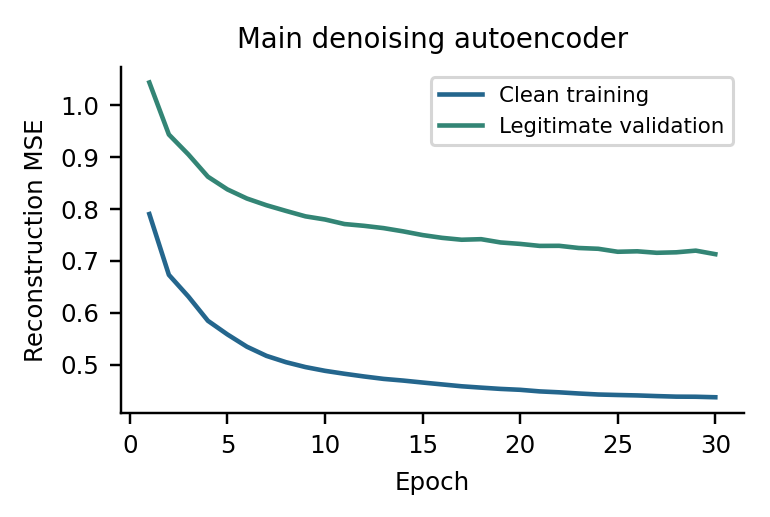
\includegraphics[width=\columnwidth]{report_learning.png}
\caption{Main denoising AE on clean inputs. It reaches the 30-epoch cap. Later validation loss can reflect distribution change as well as fit quality.}\label{fig:learning}
\end{figure}

\subsection{Technically Justified Score Fusion}
Density rarity and reconstruction difficulty are distinct anomaly questions. Their raw score units differ. Define $t_G=\operatorname{asinh}(s_G)$ and $t_A=\log(1+s_A)$. For each branch, legitimate validation scores supply median $m$ and interquartile range $q$, with a numerical floor of $10^{-8}$:
\begin{equation}
z_G=(t_G-m_G)/q_G,\quad z_A=(t_A-m_A)/q_A,
\end{equation}
\begin{equation}
s_H=0.5z_G+0.5z_A.
\end{equation}
The transformations compress extreme magnitudes; median/IQR reduces outlier sensitivity. Asinh also accepts signed GMM scores. Individual monotone transformations preserve branch rankings, while fusion can change the ordering. Equal weights are fixed without a fraud-label search. The rationale is complementary evidence, not added complexity alone. Its limitations include correlated errors and loss of a strong branch's ranking advantage. This is score-level fusion; we do not fit a GMM on the learned bottleneck.

\section{Evaluation Protocol}
For each model and $b\in\{0.001,0.005,0.01\}$, the cutoff is the normal-validation $(1-b)$ quantile using the higher observed value. The alert rule is strictly $s>\tau$. Assertions verify validation FPR at or below each budget. The default policy is $b=0.005$. Future FPR is not guaranteed by the observed validation rate. Model-specific normalization and thresholding use the same validation period, so their empirical rate is a calibration-set property, not a finite-sample future guarantee.

We report PR area using trapezoidal integration for continuity with Phase 1, and AP using recall-increment weighting. Precision is TP/(TP+FP), recall is TP/(TP+FN), and FPR is FP/(FP+TN). Precision at 100 reviews sorts test scores decreasingly, with stable ties, and counts fraud among those 100. Review capacities 50,100,200,500 refer to the whole test batch, not reviews per day. Test labels report outcomes and diagnostics only.

\section{Results and Trade-offs}
\begin{table}[!t]\centering\caption{Test ranking and ablations; top-100 column is fraud count.}\label{tab:ranking}
\begin{tabular}{lrrr}\toprule
Model & PR area & AP & Top 100\\\midrule
GMM & 0.1496 & 0.1532 & 29 \\
PCA8 & 0.0712 & 0.0729 & 6 \\
Plain AE & 0.1281 & 0.1312 & 22 \\
Denoising AE & 0.1308 & 0.1338 & 24 \\
AE bottleneck 12 & 0.1044 & 0.1068 & 13 \\
AE seed 43 & 0.0915 & 0.0938 & 12 \\
Hybrid & 0.1412 & 0.1445 & 25 \\
\bottomrule\end{tabular}\end{table}

Table~\ref{tab:ranking} shows the GMM's stronger overall ranking. Denoising AE reaches PR area 0.1308 versus GMM 0.1496. Fusion raises the AE to 0.1412 but remains below GMM. The same ordering holds for AP and precision at 100: 29\%, 24\% and 25\% for GMM, AE and hybrid. For context, 100 random reviews would contain about 0.13 frauds in expectation at this test base rate.

\begin{figure}[!t]\centering
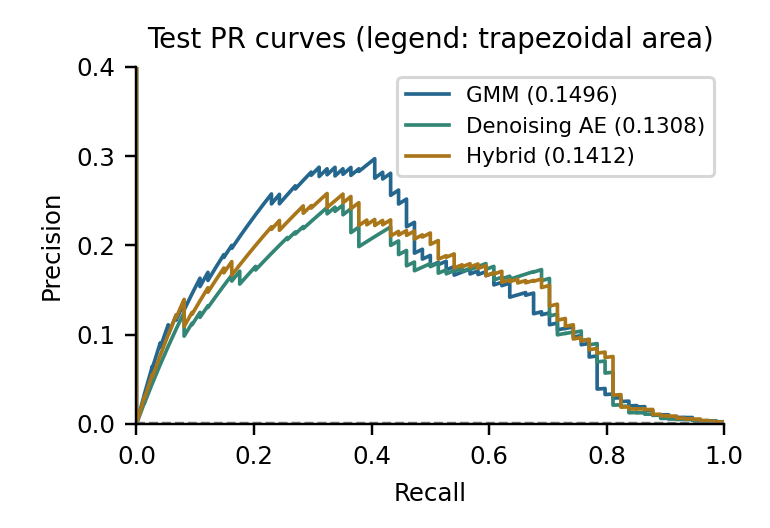
\includegraphics[width=\columnwidth]{report_pr.png}
\caption{Measured test PR curves. Equal-capacity fraud counts are in Table~\ref{tab:ranking}.}\label{fig:results}
\end{figure}

\begin{table}[!t]\centering\caption{Cutoffs set by validation FPR target, applied unchanged to test. Recall and precision are percentages.}\label{tab:policy}
\begin{tabular}{rlrrrr}\toprule
Budget\% & Model & TP & FP & Recall & Prec.\\\midrule
0.1 & GMM & 6 & 39 & 8.1 & 13.3 \\
0.1 & Denoising AE & 0 & 22 & 0.0 & 0.0 \\
0.1 & Hybrid & 0 & 25 & 0.0 & 0.0 \\
0.5 & GMM & 37 & 172 & 50.0 & 17.7 \\
0.5 & Denoising AE & 33 & 137 & 44.6 & 19.4 \\
0.5 & Hybrid & 35 & 132 & 47.3 & 21.0 \\
1.0 & GMM & 52 & 381 & 70.3 & 12.0 \\
1.0 & Denoising AE & 52 & 314 & 70.3 & 14.2 \\
1.0 & Hybrid & 52 & 304 & 70.3 & 14.6 \\
\bottomrule\end{tabular}\end{table}

At the default policy, GMM produces 209 reviews: TP=37, FP=172, FN=37, TN=56,500. AE produces 170: TP=33, FP=137, FN=41, TN=56,535. Hybrid produces 167: TP=35, FP=132, FN=39, TN=56,540. Corresponding recall is 50.00\%, 44.59\%, 47.30\%; precision is 17.70\%, 19.41\%, 20.96\%; and test FPR is 0.3035\%, 0.2417\%, 0.2329\%.

Thus hybrid has 40 fewer legitimate alerts (23.3\% fewer) than GMM but detects two fewer frauds. It detects two more than AE with five fewer false alerts. These share a validation target, not equal realized test FPR or review volume. At the 1\% validation policy, all three find 52 frauds with 381,314,304 false alerts respectively. At 0.1\%, GMM finds six frauds while AE and hybrid find none. Policy choice therefore matters. We do not retrospectively select a test-winning cutoff as a new default.

\subsection{Complementarity and Uncertainty}
GMM and AE score ranks have Spearman correlation 0.746. Among the top 100, both find the same 24 frauds, and GMM finds five additional frauds. AE contributes no unique fraud at that capacity. Equal averaging therefore loses some of the GMM ranking advantage. This diagnostic is capacity-specific and does not rule out complementary cases at other thresholds.

A paired stratified bootstrap resamples legitimate and fraud test rows separately, preserving class counts, for 200 replicates. The percentile 95\% interval for hybrid AP minus AE AP is [0.0060,0.0177]. This conditional interval ignores temporal dependence, refitting variation and benchmark reuse. It does not establish future-data or cross-seed superiority. Each of only 74 frauds changes recall by about 1.35 percentage points.

\section{Ablation Studies}
\textbf{Input noise:} Plain and denoising AE differ only in corruption SD (0 versus 0.10); training rows, seed, architecture, decay and stopping rule match. Noise raises PR area from 0.1281 to 0.1308 and top-100 frauds from 22 to 24. At the default policy both find 33, but plain AE creates fewer false alerts (127 versus 137). The benefit is metric-specific.

\textbf{Bottleneck size:} Widening 8 to 12 also increases parameters from 1,253 to 1,385. Normal-validation MSE improves from 0.7130 to 0.6599, yet PR area falls to 0.1044 and top-100 frauds to 13. Reconstruction fit and fraud ranking are different goals.

\textbf{Seed sensitivity:} Changing only the seed from 42 to 43 gives PR area 0.0915 and 12 frauds in 100 reviews. This exposes substantial sensitivity. Two seeds are a diagnostic rather than a distributional uncertainty study; the declared main seed remains fixed.

\textbf{Linear reference:} An eight-component PCA fitted on the same legitimate rows scores reconstruction MSE. It reaches PR area 0.0712 with six frauds in 100 reviews. The nonlinear AE is stronger here, while fitting methods and parameter counts differ.

\textbf{Hybrid branch removal:} GMM-only and AE-only results quantify the effect of removing each branch. GMM-only ranks best. The hybrid's operational gains at some policies do not establish a universal improvement. All weaker runs, checkpoints and histories are retained; no test-ranked ablation replaces the declared main model.

\section{Error Analysis and Limitations}
Notebook 04 shows a caught fraud, a false alert and a missed fraud at the default AE threshold, including the five largest squared feature errors. These are qualitative examples chosen after evaluation. Anonymous features permit numerical attribution but not a business explanation of stolen-card behavior.

The two-day historical dataset cannot demonstrate long-term drift resistance. The provider's PCA fitting scope is unavailable. Exact-duplicate removal is an assumption. Normal-only filtering relies on known labels. Unusual legitimate transactions and normal-looking fraud cause overlapping scores. Diagonal covariance and small model grids constrain GMM; initialization, reconstruction generalization and an unoptimized architecture constrain AE. Fusion is simple and fixed, and its gain over AE does not beat the GMM ranking. Costs, latency and analyst outcomes are not measured. This is a research comparison, not a production blocking system.

\section{Reproducibility and Team Responsibilities}
Five ordered notebooks provide shared motivation, data checks, feature scaling, AE training and final evaluation. Each starts from a fresh namespace and saves its outputs. Assertions check data identity, feature equality, finite scores, counts, validation FPR budgets and historical GMM parity. Tested versions include Python 3.12.14, NumPy 1.26.4, pandas 2.2.2, scikit-learn 1.4.2, PyTorch 2.6.0 and matplotlib 3.8.4. CPU settings and dependency versions are saved. Four AE runs require about 33 seconds of training in this workspace; total execution and fresh GMM fitting add time. Hardware can change timing and low-level numerics.

The retained responsibilities are Keshav (2401010222), data/EDA and notebook 01; Vaibhav (2401010486), features and notebook 02; Mayank (2401010267), training/ablations and notebook 03; H Maheshwari, called Hardik (2401010174), evaluation and notebook 04; and Mitul Bhatia (2401010279), leadership, integration and coordination. Mayank and Keshav retain README and presentation responsibility. All five jointly contribute to the report. These are responsibility assignments, not fabricated evidence of completed individual work. The actual-work record must be completed by members. AI assistance supported preparation; each member must verify and understand the work and follow faculty disclosure rules.

\section{Conclusion}
The DL extension successfully implements normal-only denoising reconstruction and an auditable score-fusion hybrid. GMM remains the best overall ranking model on the reused benchmark. Hybrid improves AE and can reduce false alerts compared with GMM at declared validation policies, with a recall cost at the default. Ablations show that wider bottlenecks and lower normal reconstruction error need not improve fraud detection, and that random-seed sensitivity is material. Future work should start with truly later data, more training seeds and explicit analyst costs before choosing additional complexity.

\begin{thebibliography}{00}
\bibitem{em} A. P. Dempster, N. M. Laird, and D. B. Rubin, ``Maximum likelihood from incomplete data via the EM algorithm,'' JRSS-B, 1977, doi:10.1111/j.2517-6161.1977.tb01600.x.
\bibitem{sakurada} M. Sakurada and T. Yairi, ``Anomaly detection using autoencoders with nonlinear dimensionality reduction,'' MLSDA, pp. 4--11, 2014, doi:10.1145/2689746.2689747.
\bibitem{vincent} P. Vincent et al., ``Stacked denoising autoencoders: Learning useful representations in a deep network with a local denoising criterion,'' JMLR, vol. 11, pp. 3371--3408, 2010. \url{https://www.jmlr.org/papers/v11/vincent10a.html}
\bibitem{pr} T. Saito and M. Rehmsmeier, ``The precision-recall plot is more informative than the ROC plot when evaluating binary classifiers on imbalanced datasets,'' PLOS ONE, 2015, doi:10.1371/journal.pone.0118432.
\bibitem{sk} scikit-learn, ``Average precision score,'' version 1.4.2 documentation. \url{https://scikit-learn.org/1.4/modules/generated/sklearn.metrics.average_precision_score.html}
\bibitem{torch} PyTorch, ``MSELoss'' and ``Adam,'' documentation. \url{https://docs.pytorch.org/docs/stable/generated/torch.nn.MSELoss.html}.
\bibitem{data} ULB Machine Learning Group/Worldline, ``Credit Card Fraud Detection,'' Kaggle. \url{https://www.kaggle.com/datasets/mlg-ulb/creditcardfraud}
\end{thebibliography}
\end{document}
